% debut d'un fichier latex standard
\documentclass[a4paper,12pt,twoside]{article}

% pour l'inclusion de figures en eps,pdf,jpg
\usepackage{graphicx}
\usepackage{subcaption}
\usepackage{wrapfig}
% quelques symboles mathematiques en plus
\usepackage{amsmath}
% le tout en langue francaise
%\usepackage[french]{babel}
% on peut ecrire directement les caracteres avec l'accent
% a utiliser sur Linux/Windows
\usepackage[utf8]{inputenc}
\usepackage[T1]{fontenc}
% a utiliser sur le Mac
%\usepackage[applemac]{inputenc}
% pour l'inclusion de links dans le document
\usepackage[colorlinks,bookmarks=false,linkcolor=blue,urlcolor=blue]{hyperref}
\usepackage{siunitx}

\paperheight=297mm
\paperwidth=210mm

\setlength{\textheight}{235mm}
\setlength{\topmargin}{-1.2cm} % pour centrer la page verticalement
%\setlength{\footskip}{5mm}
\setlength{\textwidth}{15cm}
\setlength{\oddsidemargin}{0.56cm}
\setlength{\evensidemargin}{0.56cm}

\pagestyle{plain}

% quelques abreviations utiles
\def \be {\begin{equation}}
\def \ee {\end{equation}}
\def \dd  {{\rm d}}

\newcommand{\mail}[1]{{\href{mailto:#1}{#1}}}
\newcommand{\ftplink}[1]{{\href{ftp://#1}{#1}}}
%
% latex SqueletteRapport.tex      % compile la source LaTeX
% xdvi SqueletteRapport.dvi &     % visualise le resultat
% dvips -t a4 -o SqueletteRapport.ps SqueletteRapport % produit un PostScript
% ps2pdf SqueletteRapport.ps      % convertit en pdf

% pdflatex SqueletteRapport.pdf    % compile et produit un pdf

% ======= Le document commence ici ======

\begin{document}
% Le titre, l'auteur et la date
\title{Heat problem\\{\small Physique Numérique I}\\{\small Rapport 5}}
\date{\today}
\author{Delphine Martres et Damien Korber\\{\small \mail{delphine.martres@epfl.ch} et \mail{damien.korber@epfl.ch}}}

\maketitle
\tableofcontents % Table des matieres


% Quelques options pour les espacements entre lignes, l'identation
% des nouveaux paragraphes, et l'espacement entre paragraphes
\baselineskip=16pt
\parindent=15pt
\parskip=5pt
\newpage


%%%% ON COMMENCE A ECRIRE D'ICI

\section{Introduction}
This project focuses on the propagation of heat in an homogeneous environment.
Two heat sources are considered: a cold and a hot one.
TODO: A COMPLETER

\section{Convergence and stability}

\begin{figure}[h]
  \centering
  \begin{subfigure}[t]{0.45\textwidth}
    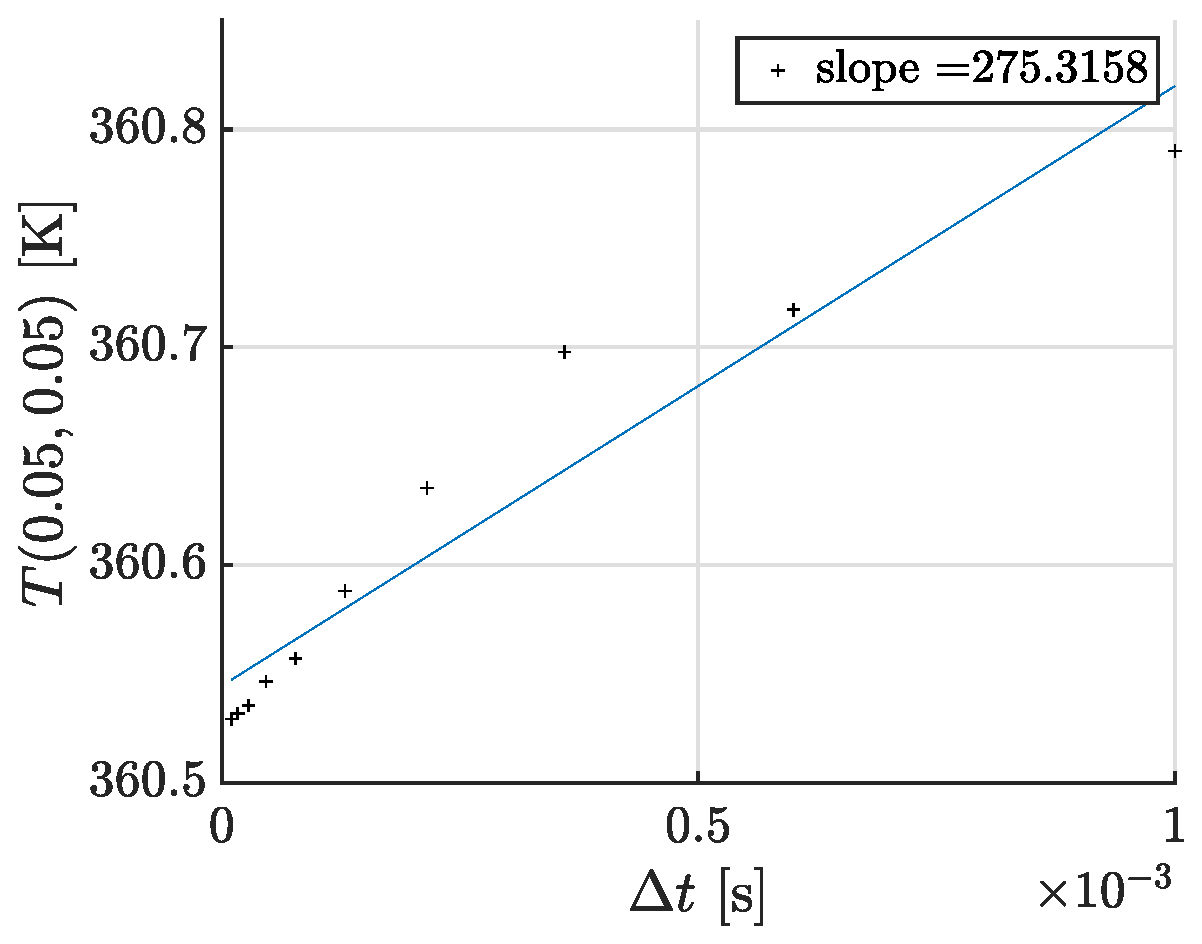
\includegraphics[width=\textwidth]{graphs/b_conv40.eps}
    
    \caption{Convergence}
    \label{fig:b-conv40}
  \end{subfigure}
  ~
  \begin{subfigure}[t]{0.45\textwidth}
    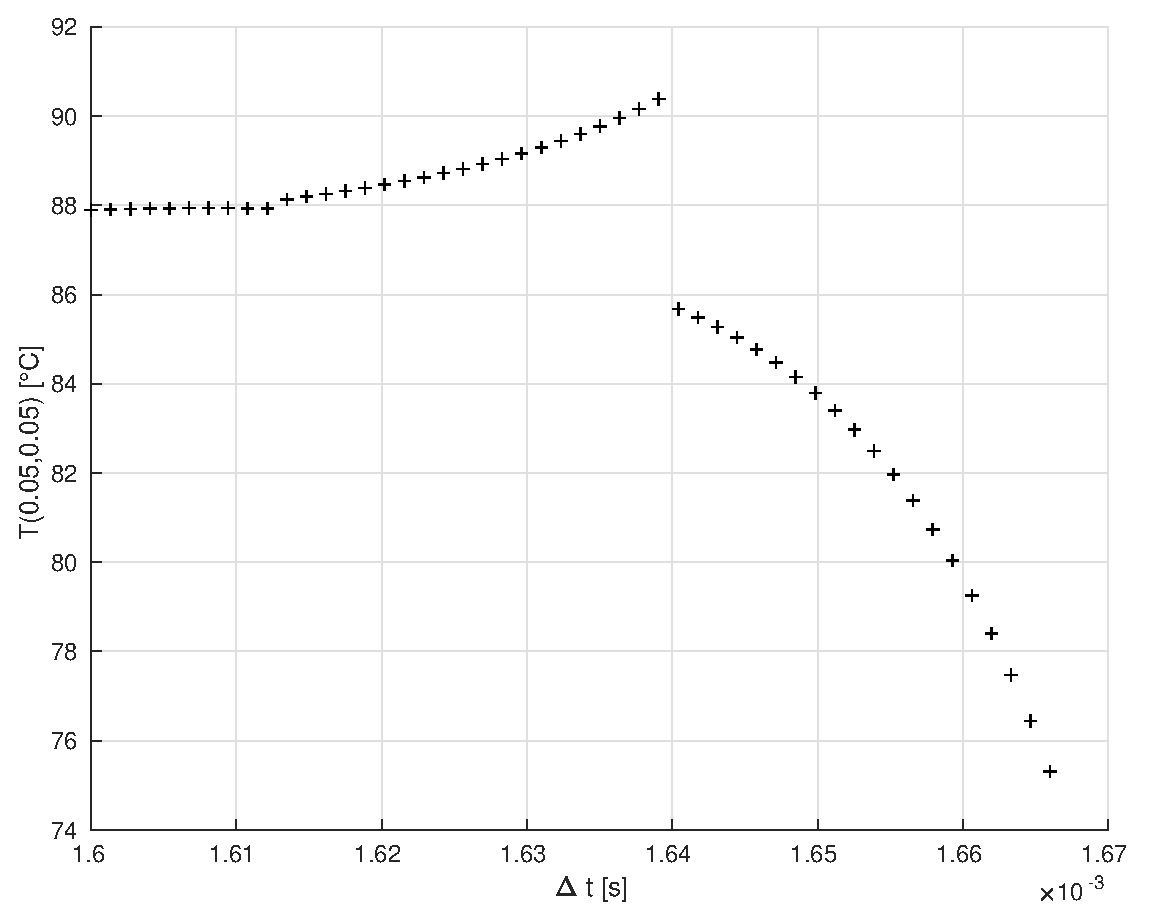
\includegraphics[width=\textwidth]{graphs/b_lim40.eps}
    \caption{Limit of stability}
    \label{fig:b-lim40}
  \end{subfigure}
  \caption{N=40}
  \label{fig:b40}
\end{figure}

\begin{figure}[h]
  \centering
  \begin{subfigure}[t]{0.45\textwidth}
    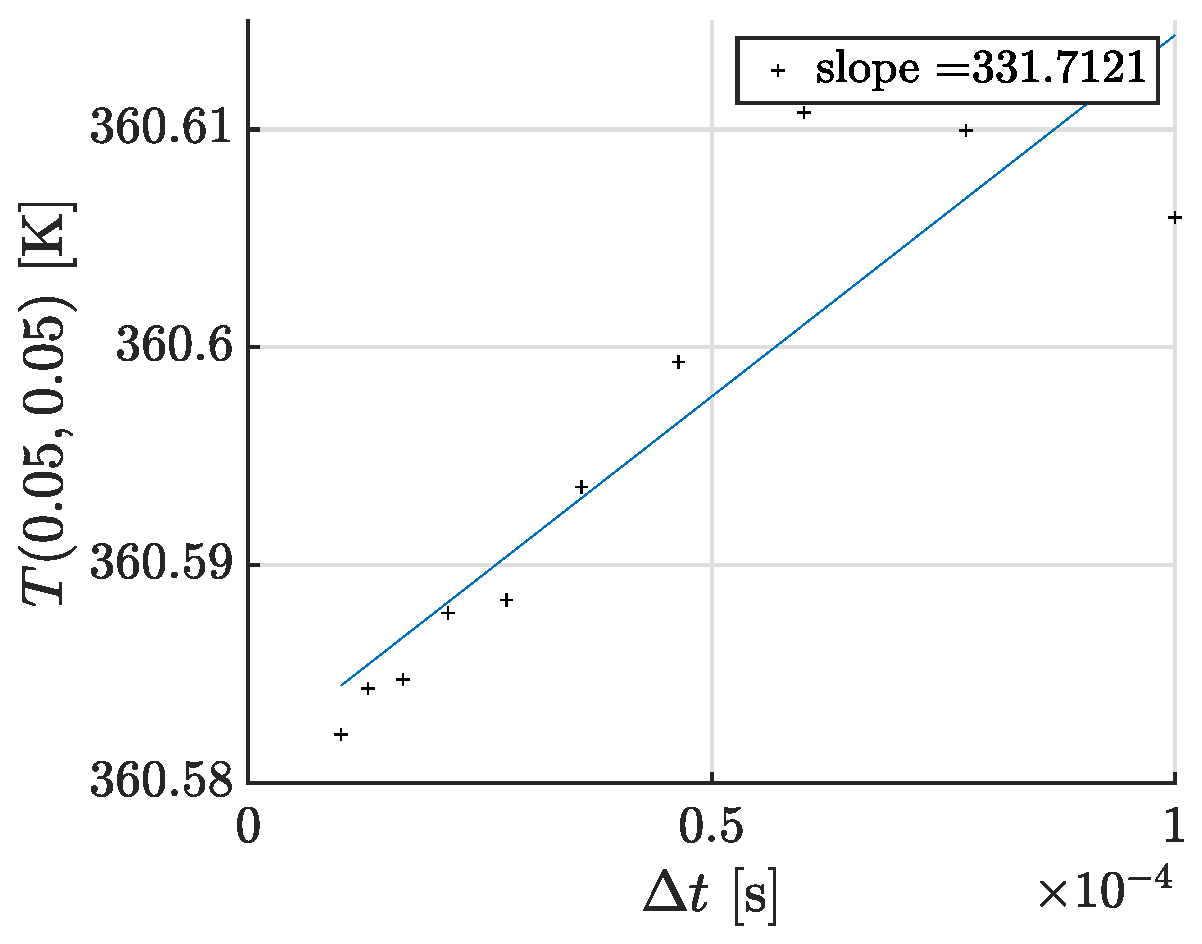
\includegraphics[width=\textwidth]{graphs/b_conv80.eps}
    
    \caption{Convergence}
    \label{fig:b-conv80}
  \end{subfigure}
  ~
  \begin{subfigure}[t]{0.45\textwidth}
    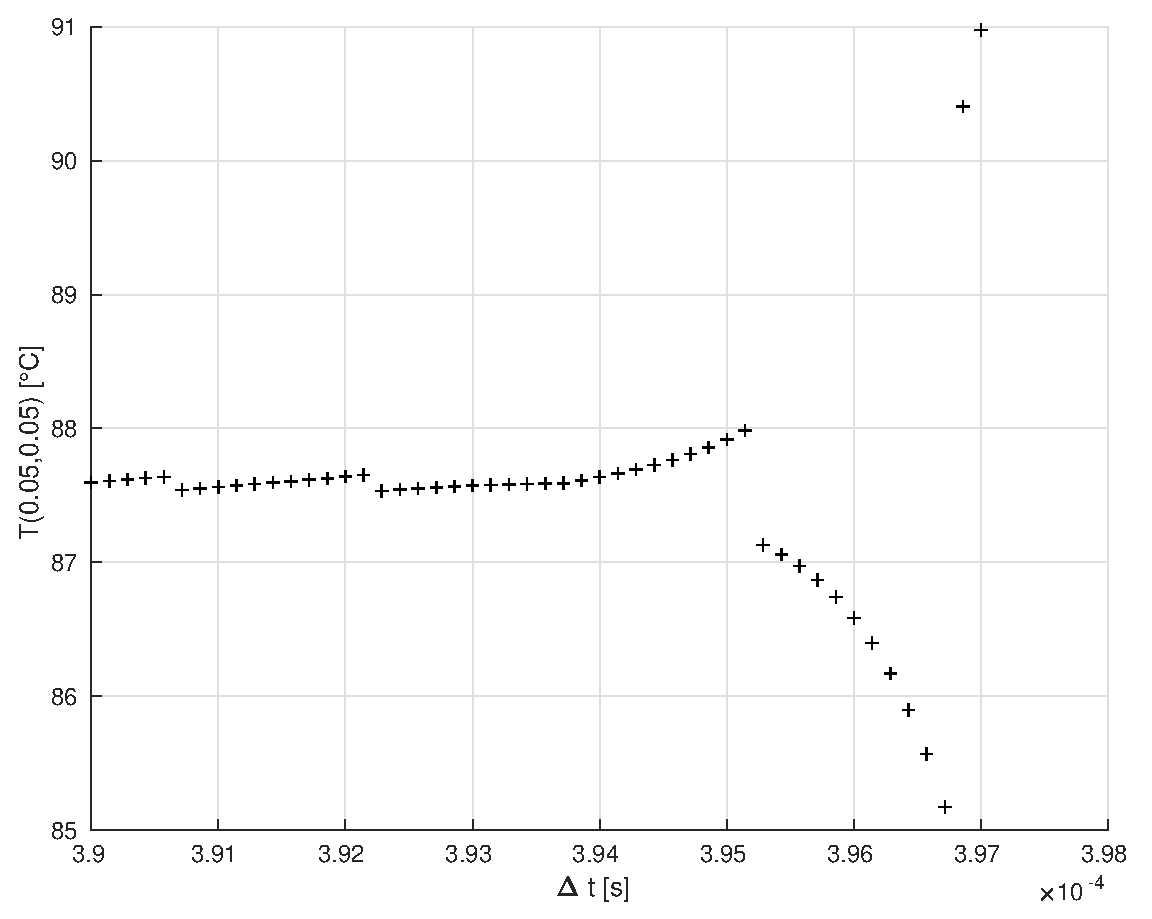
\includegraphics[width=\textwidth]{graphs/b_lim80.eps}
    \caption{Limit of stability}
    \label{fig:b-lim80}
  \end{subfigure}
  \caption{N=40}
  \label{fig:b80}
\end{figure}

\section{Heat flux}
This section focuses on the analysis of the behavious of the heat flux.
The heat flux is obtained with equation \eqref{eq:flux-chaleur}.

\begin{equation}
  \vec{j} = -\kappa\vec{\nabla} T
  \label{eq:flux-chaleur}
\end{equation}

By using a forward finite difference method, $\vec{j}$ can be numerically computed with equation \eqref{eq:flux-chaleur-numerique}.

\begin{equation}
  \vec{j} = -\frac{\kappa}{h}
  \begin{pmatrix}
    T^k_{i+1,j} - T^k_{i,j} & T^k_{i,j+1} - T^k_{i,j}
  \end{pmatrix}
  \label{eq:flux-chaleur-numerique}
\end{equation}

The result for the heat flux at $t=\SI{0.1}{\second}$ is given by figures \ref{fig:c-temp} and \ref{fig:c-heat-flux}.

\begin{figure}[h]
  \centering
  \begin{subfigure}[t]{0.45\textwidth}
    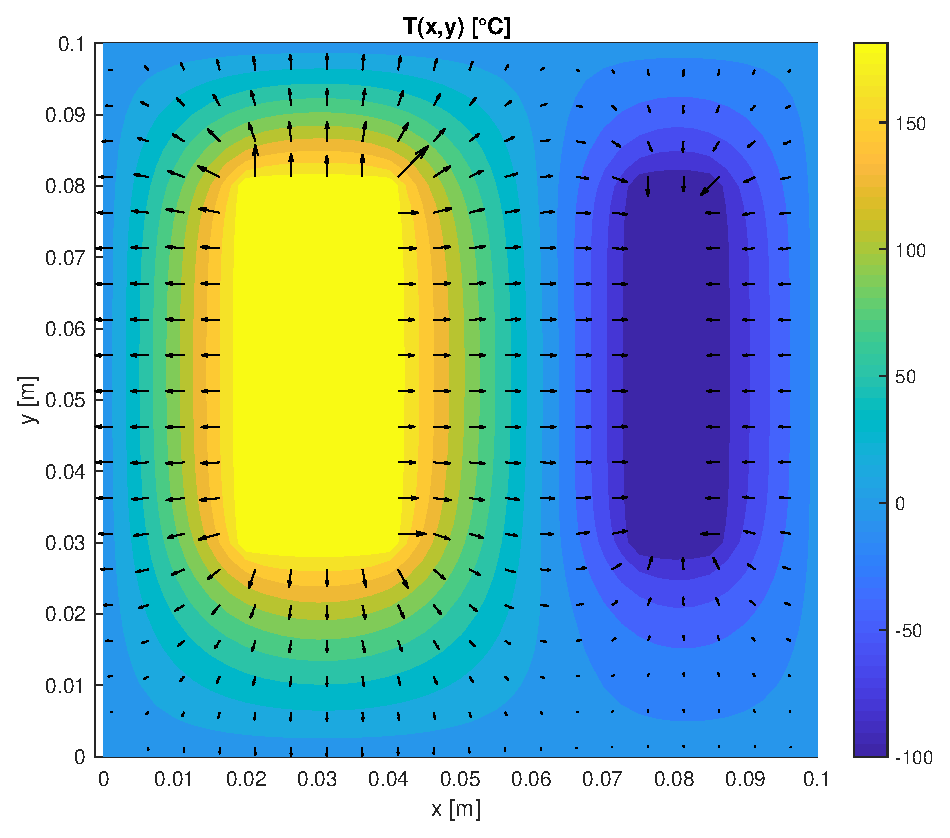
\includegraphics[width=\textwidth]{graphs/c_temp.eps}
    \caption{Graph of temperatures, represented by the color gradient, in Celsius, with the direction and the intensity of the heat flux represented by the arrows.}
    \label{fig:c-temp}
  \end{subfigure}
  ~
  \begin{subfigure}[t]{0.45\textwidth}
    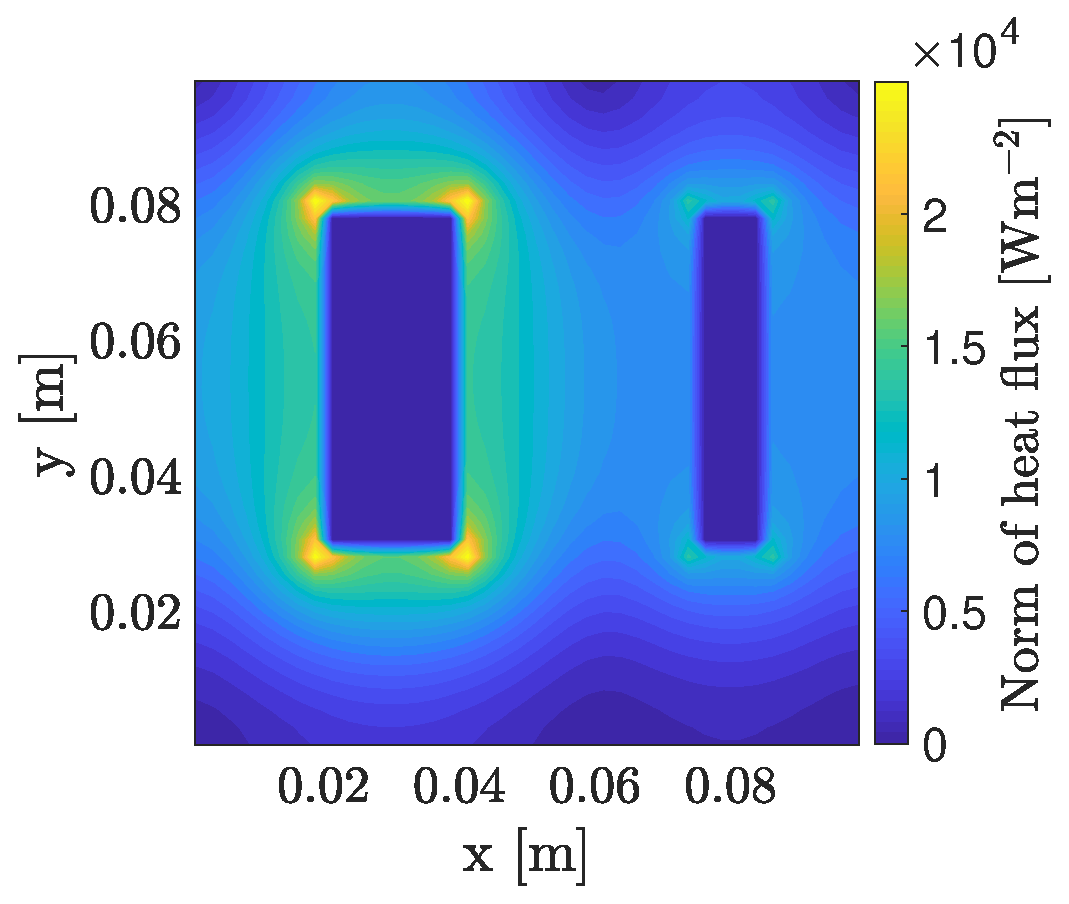
\includegraphics[width=\textwidth]{graphs/c_heat_flux.eps}
    \caption{Intensity of the heat flux represented by the color gradient.}
    \label{fig:c-heat-flux}
  \end{subfigure}
  \caption{Study of the heat flux at $t=\SI{0.1}{\second}$.}
  \label{fig:c}
\end{figure}

%TODO: ANALYSE.

\section{Power}

\section{Heat flux with respect to the distance between the bodies}

\section{Conclusion}

\end{document}
